\documentclass[12pt]{article}
\usepackage[a4paper, total={6in, 9in}]{geometry}
\usepackage{graphicx}
\graphicspath{ {./images/output/} }
\usepackage{caption}
\usepackage[english]{babel}
\usepackage{titling}
\usepackage{float}
\usepackage{amsmath}
\usepackage{minted}
% \usepackage{multicol}
% \usepackage{array}
% \usepackage{setspace}
% \usepackage{placeins}
\usepackage{parskip}

% \usepackage{lipsum}

\title{Implementation NAND Gate and NOR Gate Using CMOS}
\author{}
\date{}

\pagenumbering{gobble}
\begin{document}
\vspace*{\fill}
\begin{center}

    \emph{Heaven's Light is Our Guide} \\
    \textbf{Rajshahi University of Engineering and Technology} \\

    \begin{figure}[H]
        \centering
        
\includegraphics[scale=.34]{images/RUET_logo.png}
        \label{fig:ruet_logo}
    \end{figure}
    \vspace{5mm}

    \textbf{Course Code}\\
    ECE 4128\\
    \vspace{3mm}
    \textbf{Course Title}\\
    VLSI Design

    \vspace{5mm}
    \textbf{Experiment Date:} {July 4, 2025},\\
    \textbf{Submission Date:} {August 11, 2025}\\

    \vspace{5mm}
    \textbf{Lab Report 2: \\
        Implementation of NMOS Ratio-less Inverter.}

    \vspace{15mm}

    \begin{tabular}{c|c}
        \textbf{Submitted to} & \textbf{Submitted by} \\
        Moloy Kumar Ghosh     &                       \\
        Lecturer              &                       \\
        Dept of ECE, RUET     & Md. Tajim An Noor     \\
        \&                    & Roll: 2010025         \\
        Md. Faysal Ahamed     &                       \\
        Lecturer              &                       \\
        Dept of ECE, RUET     &                       \\
    \end{tabular}

\end{center}
\vspace*{\fill}


\pagebreak

\tableofcontents

\pagebreak
\pagenumbering{arabic}
\maketitle

\section*{Theory}
\addcontentsline{toc}{section}{Theory}
Logic gates are fundamental components in digital electronics, enabling the implementation of arithmetic, memory, and control operations within integrated circuits~\cite{weste2015cmos}. NAND and NOR gates are particularly important because they are universal gates—meaning any logic function (such as AND, OR, NOT, XOR) can be constructed using only NAND or NOR gates~\cite{manohar2017digital}. As a result, understanding the design and operation of CMOS NAND and NOR gates is essential for grasping the foundations of digital VLSI (Very Large Scale Integration) systems~\cite{kang2019cmos}.

\subsection*{CMOS Technology Overview}
\addcontentsline{toc}{subsection}{CMOS Technology Overview}
CMOS (Complementary Metal-Oxide-Semiconductor) is the predominant technology for digital circuit design, valued for its low power consumption and scalability~\cite{weste2015cmos}. CMOS circuits utilize both PMOS and NMOS transistors in a complementary configuration. The structure consists of a pull-up network (PUN) made of PMOS transistors connected to the supply voltage (VDD) and a pull-down network (PDN) of NMOS transistors connected to ground~\cite{kang2019cmos}. Inputs are applied to both networks, and the output is taken from their shared node. This arrangement ensures that, ideally, only one network conducts at a time, minimizing static power usage and producing sharp logic transitions.

\subsection*{CMOS NAND Gate}
\addcontentsline{toc}{subsection}{CMOS NAND Gate}
A CMOS NAND gate features two PMOS transistors in parallel for the pull-up network and two NMOS transistors in series for the pull-down network~\cite{weste2015cmos}. Its operation is as follows:
\begin{itemize}
    \item When both inputs are high (logic 1), both NMOS transistors conduct, creating a low-resistance path to ground and pulling the output to logic 0.
    \item For any other input combination (00, 01, or 10), at least one PMOS transistor conducts in the parallel pull-up network, pulling the output to logic 1.
\end{itemize}
This configuration matches the NAND gate truth table, with the parallel PMOS arrangement ensuring a strong pull-up except when both inputs are high.

\subsection*{CMOS NOR Gate}
\addcontentsline{toc}{subsection}{CMOS NOR Gate}
The CMOS NOR gate is the logical counterpart to the NAND gate. It uses two PMOS transistors in series for the pull-up network and two NMOS transistors in parallel for the pull-down network~\cite{kang2019cmos}. Its operation is:
\begin{itemize}
    \item When both inputs are low (logic 0), both PMOS transistors conduct, providing a path from VDD to the output and driving it to logic 1.
    \item For all other input combinations (01, 10, or 11), at least one NMOS transistor conducts in the parallel pull-down network, pulling the output to logic 0.
\end{itemize}
This setup produces the NOR gate truth table, where the output is high only when both inputs are low.

\subsection*{Advantages of CMOS NAND and NOR Gates}
\addcontentsline{toc}{subsection}{Advantages of CMOS NAND and NOR Gates}
CMOS implementations of NAND and NOR gates offer several benefits. The complementary design results in minimal static power dissipation, as there is no direct path from VDD to ground except during switching~\cite{manohar2017digital}. CMOS gates also provide high noise immunity, sharp switching thresholds, and are easily scalable with modern fabrication techniques~\cite{weste2015cmos}. Their universality makes NAND and NOR gates essential building blocks for more complex logic circuits, underscoring their importance in VLSI and digital system design~\cite{kang2019cmos}.

\section*{Required Tools}
\addcontentsline{toc}{section}{Required Tools}
\begin{itemize}
    \item Microwind
    \item MS Word
    \item \LaTeX
\end{itemize}

\section*{Circuit Schematic}
\addcontentsline{toc}{section}{Circuit Schematic}

\begin{figure}[H]
    \centering
    \begin{minipage}{0.48\textwidth}
        \centering
        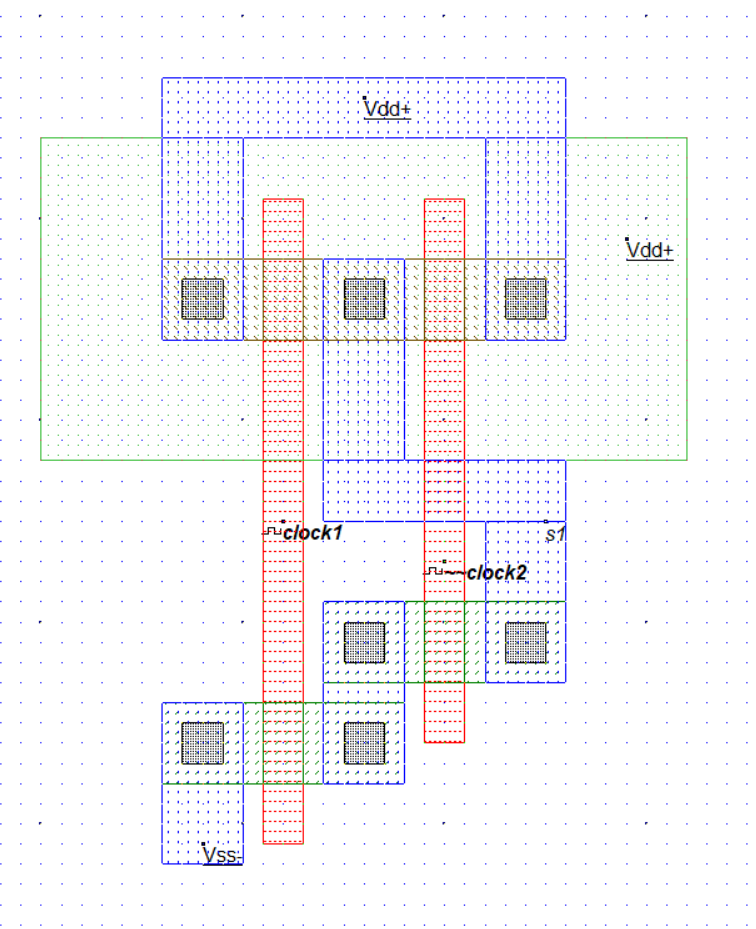
\includegraphics[width=\textwidth]{3Nand.png}
        \caption{CMOS NAND Gate Schematic}
    \end{minipage}\hfill
    \begin{minipage}{0.48\textwidth}
        \centering
        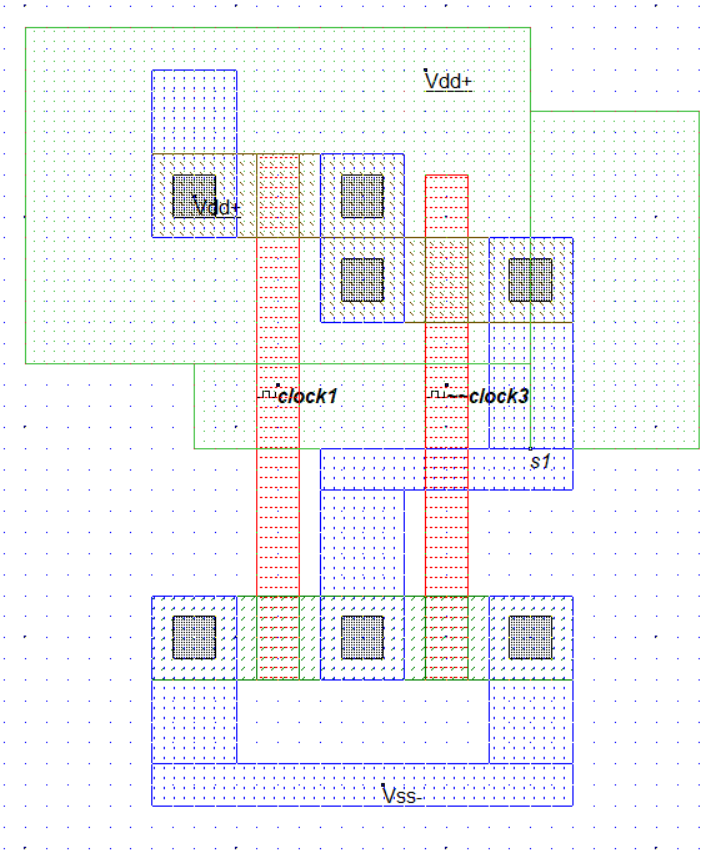
\includegraphics[width=\textwidth]{3Nor.png}
        \caption{CMOS NOR Gate Schematic}
    \end{minipage}
\end{figure}

\section*{Output}
\addcontentsline{toc}{section}{Output}

\begin{figure}[H]
    \centering
    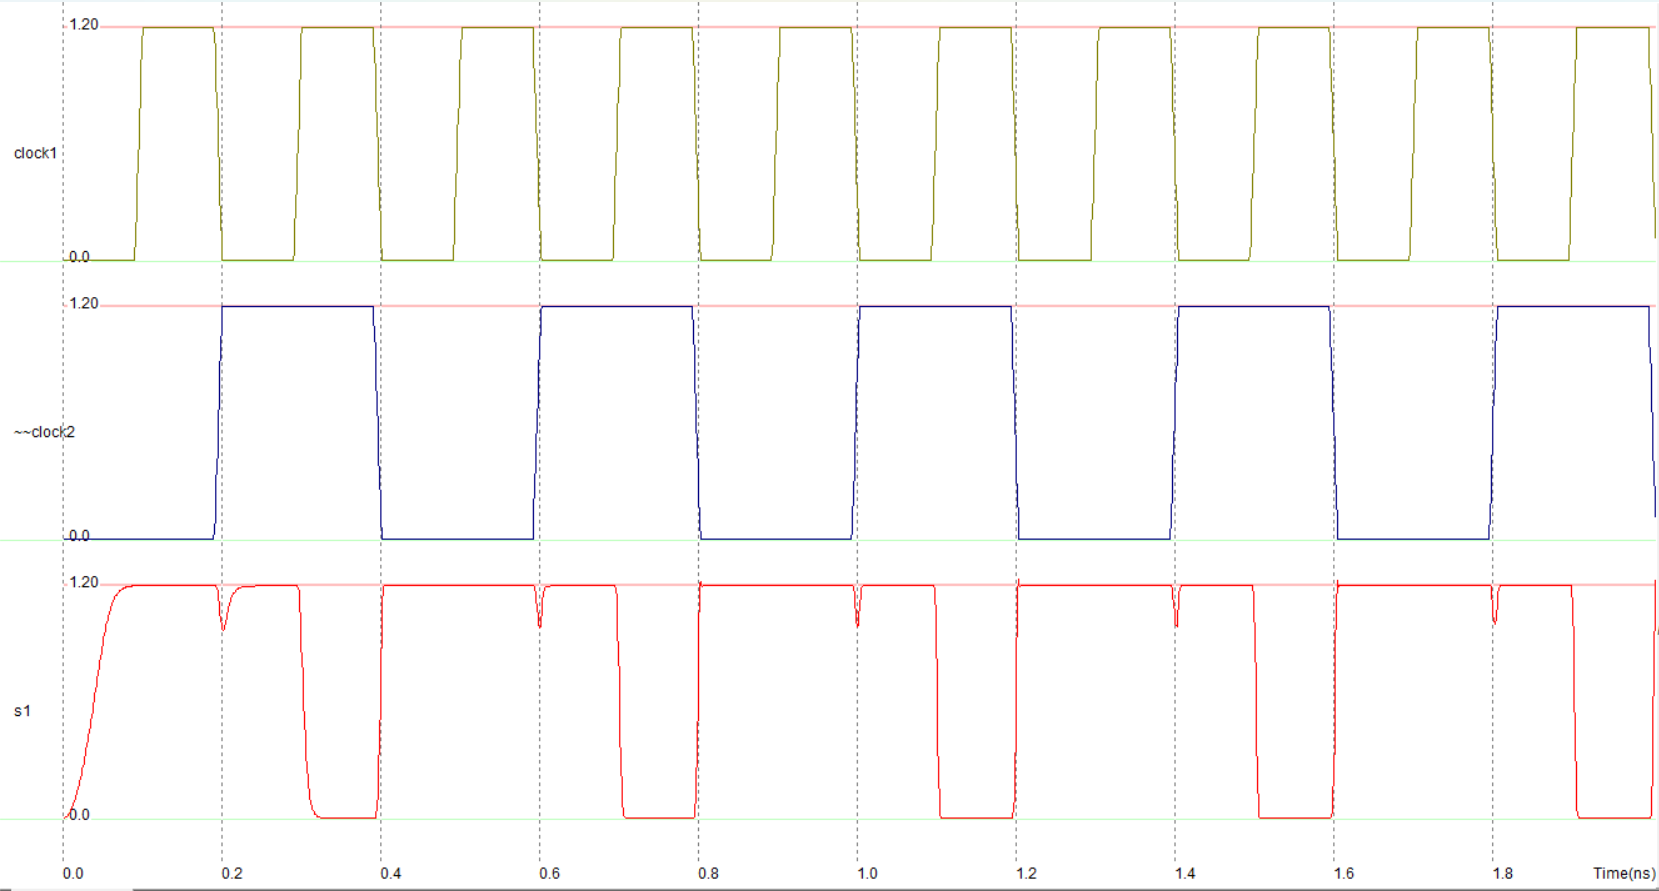
\includegraphics[width=0.8\textwidth]{3Nand_tt.png}
    \caption{Output Waveform of CMOS NAND Gate}
\end{figure}

\begin{figure}[H]
    \centering
    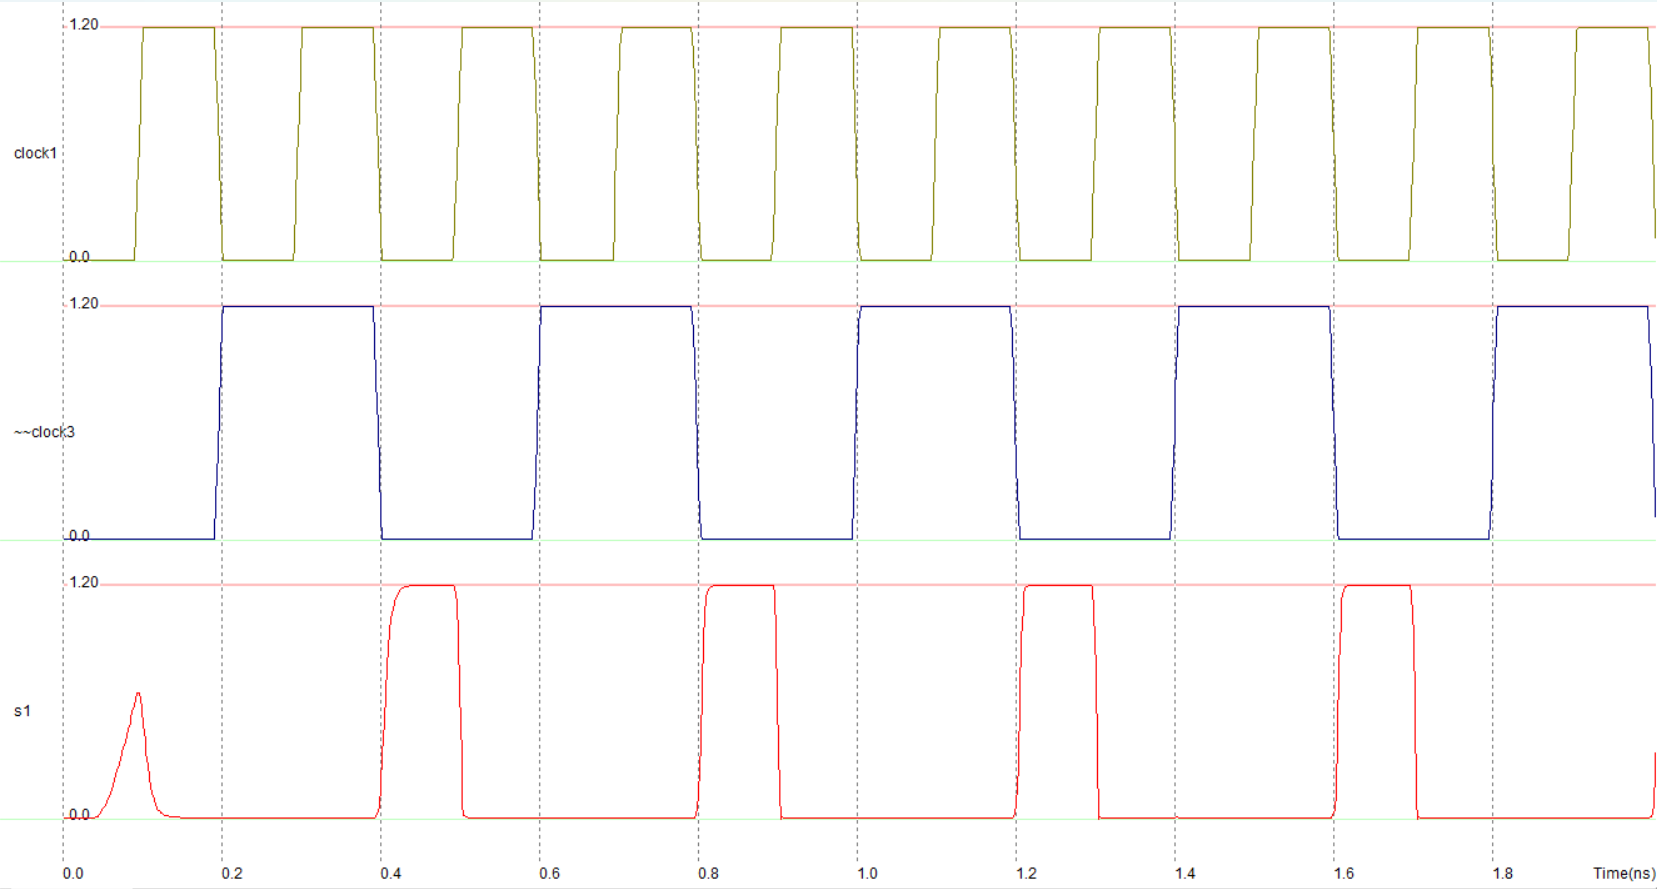
\includegraphics[width=0.8\textwidth]{3Nor_tt.png}
    \caption{Output Waveform of CMOS NOR Gate}
\end{figure}

\subsection*{Output Analysis}
\addcontentsline{toc}{subsection}{Output Analysis}

\textbf{NOR Gate:} \\
The output signal \texttt{s1} is high only when both \texttt{clock1} and \texttt{clock3} are at logic 0. If either input is at logic 1, \texttt{s1} transitions low, which is consistent with the NOR gate truth table. The waveform segments correspond to the following input combinations:
\begin{itemize}
    \item (0,0): \texttt{s1} = 1
    \item (1,0), (0,1), (1,1): \texttt{s1} = 0
\end{itemize}

\textbf{NAND Gate:} \\
The output \texttt{s1} is low only when both \texttt{clock1} and \texttt{clock2} are at logic 1. For all other input combinations, \texttt{s1} remains high, matching the NAND gate truth table. The waveform mapping is as follows:
\begin{itemize}
    \item (1,1): \texttt{s1} = 0
    \item (0,0), (0,1), (1,0): \texttt{s1} = 1
\end{itemize}

\section*{Discussion and Conclusion}
\addcontentsline{toc}{section}{Discussion and Conclusion}
In this experiment, CMOS NAND and NOR gates were implemented and simulated to observe their logical behavior. The simulation results aligned with the theoretical truth tables: the NAND gate produced a low output only when both inputs were high, and the NOR gate generated a high output only when both inputs were low. These outcomes verified the correct functioning of the complementary pull-up and pull-down networks in CMOS logic circuits.

The simulation further demonstrated the efficiency of CMOS technology. Static power dissipation was minimal, as only one network (either pull-up or pull-down) was active at any given time, with transient power consumption occurring during input transitions. The configuration of PMOS and NMOS transistors—whether in series or parallel—determined both the logic operation and the robustness of output transitions.

In summary, the experiment confirmed the theoretical foundations of CMOS logic design, highlighting its advantages in low power consumption, noise immunity, and scalability. It also underscored the significance of NAND and NOR gates as universal elements for constructing complex digital systems.

\bibliographystyle{IEEEtran}
\renewcommand{\bibname}{References}
\addcontentsline{toc}{section}{References}
\bibliography{ref}

\end{document}
